\section{Sensor Placement for Optimal Coverage: Formulations}
Let $\mathcal E \subset \mathbb R^3$ be a bounded three-dimensional workspace that is path-connected, e.g., a hilly terrain or an intensive care unit (ICU) in a hospital. We consider the problem of deploying $k$ ``mobile sensors'', $c_1, \ldots, c_k$, to guard a \emph{critical subset} $S$ embedded in the surface of $\mathcal E$, i.e., $S \subset \partial \mathcal E$ where $\partial$ is the boundary operator. For example, if $\mathcal E$ is a hospital ICU, $S$ may be a part of its interior surface. The sensors are to be deployed to achieve a globally optimal coverage of $S$ satisfying some prescribed objective, to be made more precise as the problems are further grounded for specific sensor models. We denote this broad class of problems as \emph{Sensor Placement for Optimal Coverage} (\spoc). 
%

The terms \emph{mobile sensor} and \emph{coverage} are used in a broad sense. Beyond traditional sensors that only collect information, we are interested in mobile robots with means to effect the environment as well. For example, a mobile robot may be equipped with a disinfecting light source (e.g., UVC) for eradicating harmful microbes (e.g., viruses and bacteria). Nevertheless, such settings can be nicely captured under a general sensor coverage formulation. 

In this study, we explore two common types of coverage models: \emph{visibility}-based and \emph{quality}-based. 
%
In a \emph{visibility}-based sensor coverage model, as the term suggests, a point $p \in S$ is considered covered by a sensor $c$ if $p$ is visible from $c$.
%, i.e., the straight line path between $p$ and $c$ does not intersect the 3D environment $\mathcal E$. 
When there is more than one sensor, a point $p$ is covered if it is visible from any sensor $c_i \in \{c_1, \ldots, c_k\}$. 
%
In a \emph{quality}-based model, the coverage quality of a point $p \in S$ is captured by some function that potentially depends on the sensors, the point $p$, and its neighborhood in $S$. For example, one type of quality measurement can be based on the inverse of the distance between a point $p$ and its closest sensor $c$. 

Formally, we capture the different sensor models under a unified function $f(c_1, \ldots, c_k, p, \mathcal E)$ whose co-domain is non-negative real, i.e., $f: \mathbb R^{3k + 3} \times \mathcal E \to \mathbb R_+\cup\{0\}$. In what follows, $\mathcal E$ is omitted but understood to be part of the input to $f$. In this chapter, the following instantiations are considered:
\begin{itemize}[leftmargin=4mm]
    \item Let $vis(p, c) = 1$ if the point $p$ is visible to the sensor $c$. Otherwise, $vis(p, c) = 0$. For example, an omni-directional visibility model would have $vis(p, c) = 1$ if the open line segment between $p$ and $c$ does not intersect $\mathcal E$. In a model based purely on \textbf{visibility},  
    \begin{align}
    f(c_1, \ldots, c_k, p) := \max_{1\le i \le k}vis(p, c_i).\label{f:surf-1}
    \end{align}
    \item Let the \emph{coverage quality} of a point $p$ by a sensor $c_i$ be represented as a function $\phi(p, c_i) \in \mathbb R_+\cup\{0\}$. In a \textbf{quality maximization} sensor model,  the coverage quality for a point $p$ is determined by a single best sensor:  
    \begin{align}f(c_1, \ldots, c_k, p) := \max_{1\le i \le k} \phi(p, c_i)vis(p, c_i).\label{f:surf-2}
    \end{align}
    \item In a \textbf{cumulative quality} sensor model, the overall quality of coverage at a point $p$ is the sum of the effects of all visible sensors:
    \begin{align}f(c_1, \ldots, c_k, p) := \sum_{1\le i \le k}\phi(p, c_i)vis(p, c_i).\label{f:surf-3}
    \end{align}
\end{itemize}

All the above models have direct and practical applications. 
A visibility model is applicable to the deployment of a network of $360^{\circ}$ cameras for monitoring. 
Letting $\phi(p, c_i) = \lVert pc_i\rVert^{-1}$ ($\lVert pc_i\rVert$ denotes the distance between $p$ and $c_i$), 
the quality maximization model becomes the $k$-center problem \cite{weber1929theory} if we optimize $\min_p f(c_1, \ldots, c_k, p)$, 
a broadly applicable problem. For the cumulative quality model, when the ``sensors'' are UVC lights, 
one may ask the question of how to optimally place these lights to ensure the highest percentage of $S$ can be exposed to sufficient UVC light for eradicating SARS-CoV-2 and other microbes. 
Here, a cumulative quality model clearly makes sense. 

To fully ground the discussion that follows, we formulate three concrete optimization problems, one for each of the above-mentioned sensor models. 

\begin{problem}[Visibility Maximization]\label{p:surf-1} 
    Given $S \subset \partial \mathcal E$ with $\mathcal E \subset \mathbb R^{3}$, $c_i \in \mathbb R^3$, 
    $1 \le i \le k$, and $f(c_1, \ldots, c_k, p)$ from \eqref{f:surf-1}, 
    determine a placement of $c_1, \ldots, c_k$ that maximizes the \ul{support of $f$}, i.e., 
    $supp(f) = \{p \in S \mid \max_{1\le i \le k}vis(p, c_i) >0\}.$  
\end{problem}

\begin{problem}[Quality Maximization]\label{p:surf-2} 
    Given $S \subset \partial \mathcal E$ with $\mathcal E \subset \mathbb R^{3}$, $c_i \in \mathbb R^3$, 
    $1 \le i \le k$, and $f(c_1, \ldots, c_k, p)$ from \eqref{f:surf-2} with $\phi(p, c_i) = \lVert pc_i\rVert^{-1}$, 
    determine a placement of $c_1, \ldots, c_k$ that maximizes the \ul{minimum coverage quality}, i.e., 
    $\min_{p \in S} \max_{1\le i \le k} \frac{vis(p, c_i)}{ \lVert pc_i\rVert}.$
\end{problem}

\begin{problem}[Cumulative Quality]\label{p:surf-3} 
    Given $S \subset \partial \mathcal E$ with $\mathcal E \subset \mathbb R^{3}$, 
    $c_i \in \mathbb R^3$, $1 \le i \le k$, and $f(c_1, \ldots, c_k, p)$ from \eqref{f:surf-3} with $\phi(p, c_i) = |lVert pc_i \rVert^{-2}\langle \hat{n}_p, \hat{n}_{pc_i} \rangle$ where $\hat{n}_p$ is the unit normal of $S$ at $p$ and $\hat{n}_{pc_i}$ is the unit vector in the direction from $p$ to $c_i$, 
    determine a placement of $c_1, \ldots, c_k$ that maximizes the \ul{coverage area where $f$ is above a given threshold} $\Phi > 0$,
    $supp(f - \Phi) = \{p \in S \mid \sum_{1\le i \le k} \frac{vis(p, c_i)\langle \hat{n}_p, \hat{n}_{pc_i} \rangle}{ \lVert pc_i \rVert ^2} > \Phi \}.$  
\end{problem}


\begin{wrapfigure}{r}{1.4in}
%   \vspace*{-1mm}
  \begin{overpic}[width=1.4in]{chapters/surf/fig/exposure.png}
	\end{overpic}
% \vspace*{-3.5mm}
\caption[Surface exposure]{For a point with the normal shown as the arrow, light sources on the same dotted curve provide the same level of exposure.}
\label{fig:surf-exposure}
\end{wrapfigure}
An implicit assumption for Problem~\ref{p:surf-2} to be meaningful is that an arbitrary $p \in S$ is visible to the closest sensor, 
which limits the choice of $S$. Problem~\ref{p:surf-2} is a suitable model for, 
e.g., surveillance applications that cannot tolerate any blind spots. 
A generalization with less limitation can require a certain percentage of $S$, e.g., $80\%$, to have optimized coverage. 
Problem~\ref{p:surf-3}, which computes coverage quality using the formula  $\langle \hat{n}_p, \hat{n}_{pc_i} \rangle \lVert pc_i\rVert^{-2}$, 
takes after a standard light exposure model that depends on the inverse of the squared distance and incoming light angle with respect to a local surface region (see ~\ref{fig:surf-exposure}). 

A 2D illustration of the three models is given in ~\ref{fig:surf-models}. 

\begin{figure}[ht]
    \vspace{1mm}
\centering
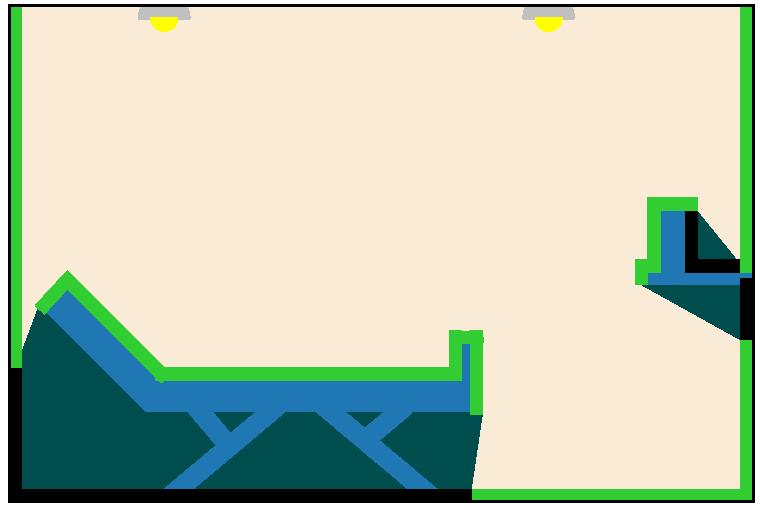
\includegraphics[width=0.305\textwidth]{chapters/surf/fig/model1-eps-converted-to.pdf}
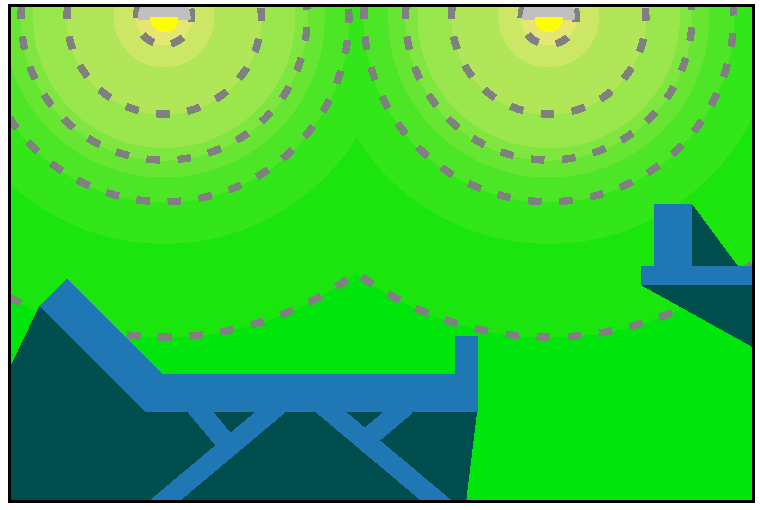
\includegraphics[width=0.305\textwidth]{chapters/surf/fig/model2-eps-converted-to.pdf}
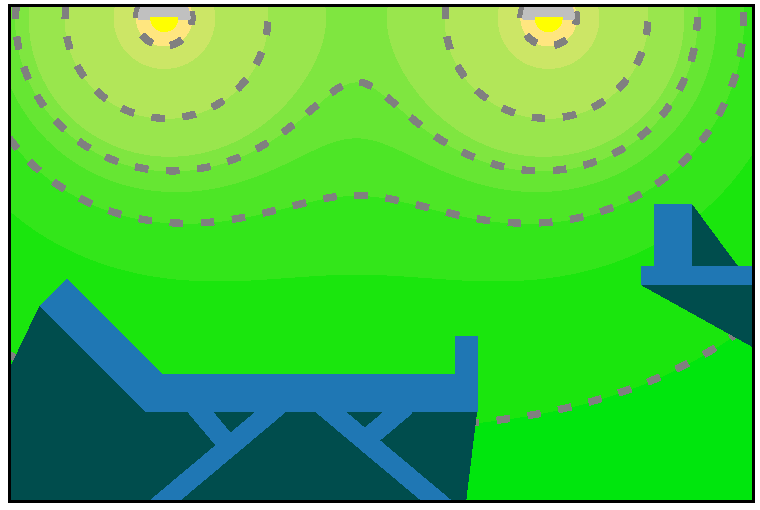
\includegraphics[width=0.305\textwidth]{chapters/surf/fig/model3-eps-converted-to.pdf}
\centering
    \vspace{1mm}
\caption[Illustration of the effects of two sensors]{Illustration of the effects of two sensors (or light sources) under three different models. \
    Only a 2D slice of a simple ICU with a bed and a counter is shown for clarity. \
    [left] A visibility-based sensing model where the green segments show the visible surfaces. \
    [middle] A quality maximization model where the dotted lines show the equal-quality level sets. \
    $\phi(p, c_i) = \lVert pc_i\rVert^{-1}$ [right] A cumulative quality model with \
    $\phi(p, c_i) = \lVert pc_i\rVert^{-2}\langle \hat{n}_p, \hat{n}_{pc_i} \rangle$. \
    Again, the dotted lines show the additive quality. The impact of the surface normal is not displayed in the figure.} 
    \label{fig:surf-models}
\end{figure}

Problems~\ref{p:surf-1}-\ref{p:surf-3} allow sensor locations to be anywhere in $\mathcal E$. 
In practice, sensor locations are often limited to a 2D surface. 
For example, in a museum or a bus, cameras are mounted on walls and ceilings. 
For drones surveying an area, there is often a preferred height to fly at. 
With this in mind, whereas the algorithms we develop are general, 
the evaluation is mainly focused on practical settings where sensor locations are confined to some plane (e.g., the roof of a room).
